%===============================================================================
% LaTeX sjabloon voor de bachelorproef toegepaste informatica aan HOGENT
% Meer info op https://github.com/HoGentTIN/latex-hogent-report
%===============================================================================

\documentclass[dutch,dit,thesis]{hogentreport}


% TODO:
% - If necessary, replace the option `dit`' with your own department!
%   Valid entries are dbo, dbt, dgz, dit, dlo, dog, dsa, soa
% - If you write your thesis in English (remark: only possible after getting
%   explicit approval!), remove the option "dutch," or replace with "english".

\usepackage{lipsum} % For blind text, can be removed after adding actual content
\usepackage[backend=biber,style=apa]{biblatex}

%% Pictures to include in the text can be put isn the graphics/ folder
\graphicspath{{graphics/}}

%% For source code highlighting, requires pygments to be installed
%% Compile with the -shell-escape flag!
\usepackage[section]{minted}
\usepackage{amsmath}
\usepackage{enumitem}
\usepackage{listings}
\usepackage{xcolor}
\definecolor{backcolour}{rgb}{0.95,0.95,0.92}
\definecolor{hogent-darkgreen}{RGB}{22,176,165}
\definecolor{hogent-pink}{RGB}{241,157,160}
\definecolor{hogent-ochre}{RGB}{250,188,50}
\definecolor{hogent-orange}{RGB}{239,135,103}
\definecolor{hogent-purple}{RGB}{187,144,189}
\definecolor{hogent-blue}{RGB}{76,162,213}
\definecolor{hogent-lightgreen}{RGB}{165,202,114}
\definecolor{hogent-brown}{RGB}{216,176,131}
\definecolor{hogent-grey}{RGB}{195,187,175}
\definecolor{hogent-yellow}{RGB}{244,222,0}

\lstdefinestyle{mystyle}{
    backgroundcolor=\color{backcolour},   
    commentstyle=\color{hogent-darkgreen},
    keywordstyle=\color{hogent-purple},
    numberstyle=\tiny\color{hogent-grey},
    stringstyle=\color{codepurple},
    caption={\color{hogent-blue}{\protect\caption}},
    basicstyle=\ttfamily\footnotesize,
    breakatwhitespace=false,         
    breaklines=true,                 
    captionpos=b,                    
    keepspaces=true,                 
    numbers=left,                    
    numbersep=5pt,                  
    showspaces=false,                
    showstringspaces=false,
    showtabs=false,                  
    tabsize=2
}

\lstset{style=mystyle}


%% If you compile with the make_thesis.{bat,sh} script, use the following
%% import instead:
%% \usepackage[section,outputdir=../output]{minted}
\usemintedstyle{solarized-light}
\definecolor{bg}{RGB}{253,246,227} %% Set the background color of the codeframe

%% Change this line to edit the line numbering style:
\renewcommand{\theFancyVerbLine}{\ttfamily\scriptsize\arabic{FancyVerbLine}}

%% Macro definition to load external java source files with \javacode{filename}:
\newmintedfile[javacode]{java}{
    bgcolor=bg,
    fontfamily=tt,
    linenos=true,
    numberblanklines=true,
    numbersep=5pt,
    gobble=0,
    framesep=2mm,
    funcnamehighlighting=true,
    tabsize=4,
    obeytabs=false,
    breaklines=true,
    mathescape=false
    samepage=false,
    showspaces=false,
    showtabs =false,
    texcl=false,
}

% Other packages not already included can be imported here

%%---------- Document metadata -------------------------------------------------
% TODO: Replace this with your own information
\author{Alexandra Stalmans}
\supervisor{Mevr. C. De Leenheer}
\cosupervisor{Dhr. T. Sanglet}
\title[]%
{Machine Learning pipeline voor Facial Image Analysis in camera-gebaseerde gezondheidsmetingen: Schatten van leeftijd en geslacht voor het beoordelen van geestelijke gezondheid}
\academicyear{\advance\year by -1 \the\year--\advance\year by 1 \the\year}
\examperiod{1}
\degreesought{\IfLanguageName{dutch}{Professionele bachelor in de toegepaste informatica}{Bachelor of applied computer science}}
\partialthesis{false} %% To display 'in partial fulfilment'
%\institution{Internshipcompany BVBA.}

%% Add global exceptions to the hyphenation here
\hyphenation{back-slash}

% The bibliography (style and settings are  found in hogentthesis.cls)

\addbibresource{../bachproef/bachproef.bib}
\addbibresource{../voorstel/voorstel.bib} %% Bibliography research proposal
\defbibheading{bibempty}{}

%% Prevent empty pages for right-handed chapter starts in twoside mode
\renewcommand{\cleardoublepage}{\clearpage}

\renewcommand{\arraystretch}{1.2}

%% Content starts here.
\begin{document}
    
    %---------- Front matter -------------------------------------------------------
    
    \frontmatter
    
    \hypersetup{pageanchor=false} %% Disable page numbering references
    %% Render a Dutch outer title page if the main language is English
    \IfLanguageName{english}{%
        %% If necessary, information can be changed here
        \degreesought{Professionele Bachelor toegepaste informatica}%
        \begin{otherlanguage}{dutch}%
            \maketitle%
        \end{otherlanguage}%
    }{}
    
    %% Generates title page content
    \maketitle
    \hypersetup{pageanchor=true}
    
    %%=============================================================================
%% Voorwoord
%%=============================================================================

\chapter*{\IfLanguageName{dutch}{Woord vooraf}{Preface}}%
\label{ch:voorwoord}

%% TODO:
%% Het voorwoord is het enige deel van de bachelorproef waar je vanuit je
%% eigen standpunt (``ik-vorm'') mag schrijven. Je kan hier bv. motiveren
%% waarom jij het onderwerp wil bespreken.
%% Vergeet ook niet te bedanken wie je geholpen/gesteund/... heeft

\lipsum[1-2]
    %%=============================================================================
%% Samenvatting
%%=============================================================================

% TODO: De "abstract" of samenvatting is een kernachtige (~ 1 blz. voor een
% thesis) synthese van het document.
%
% Een goede abstract biedt een kernachtig antwoord op volgende vragen:
%
% 1. Waarover gaat de bachelorproef?
% 2. Waarom heb je er over geschreven?
% 3. Hoe heb je het onderzoek uitgevoerd?
% 4. Wat waren de resultaten? Wat blijkt uit je onderzoek?
% 5. Wat betekenen je resultaten? Wat is de relevantie voor het werkveld?
%
% Daarom bestaat een abstract uit volgende componenten:
%
% - inleiding + kaderen thema
% - probleemstelling
% - (centrale) onderzoeksvraag
% - onderzoeksdoelstelling
% - methodologie
% - resultaten (beperk tot de belangrijkste, relevant voor de onderzoeksvraag)
% - conclusies, aanbevelingen, beperkingen
%
% LET OP! Een samenvatting is GEEN voorwoord!

%%---------- Nederlandse samenvatting -----------------------------------------
%
% TODO: Als je je bachelorproef in het Engels schrijft, moet je eerst een
% Nederlandse samenvatting invoegen. Haal daarvoor onderstaande code uit
% commentaar.
% Wie zijn bachelorproef in het Nederlands schrijft, kan dit negeren, de inhoud
% wordt niet in het document ingevoegd.

\IfLanguageName{english}{%
\selectlanguage{dutch}
\chapter*{Samenvatting}
\lipsum[1-4]
\selectlanguage{english}
}{}

%%---------- Samenvatting -----------------------------------------------------
% De samenvatting in de hoofdtaal van het document

\chapter*{\IfLanguageName{dutch}{Samenvatting}{Abstract}}

\lipsum[1-4]

    
    %---------- Inhoud, lijst figuren, ... -----------------------------------------
    
    \tableofcontents
    
    % In a list of figures, the complete caption will be included. To prevent this,
    % ALWAYS add a short description in the caption!
    %
    %  \caption[short description]{elaborate description}
    %
    % If you do, only the short description will be used in the list of figures
    
    \listoffigures
    
    % If you included tables and/or source code listings, uncomment the appropriate
    % lines.
    %\listoftables
    \listoflistings
    
    % Als je een lijst van ingeingen of termen wil toevoegen, dan hoort die
    % hier thuis. Gebruik bijvoorbeeld de ``glossaries'' package.
    % https://www.overleaf.com/learn/latex/Glossaries
    
    
    %---------- Kern ---------------------------------------------------------------
    
    \mainmatter{}
    
    % De eerste hoofdstukken van een bachelorproef zijn meestal een inleiding op
    % het onderwerp, literatuurstudie en verantwoording methodologie.
    % Aarzel niet om een meer beschrijvende titel aan deze hoofdstukken te geven of
    % om bijvoorbeeld de inleiding en/of stand van zaken over meerdere hoofdstukken
    % te verspreiden!

    
    
    %%=============================================================================
%% Inleiding
%%=============================================================================

\chapter{\IfLanguageName{dutch}{Inleiding}{Introduction}}%
\label{ch:inleiding}

De onderzoeksvraag werd aangeboden door het bedrijf IntelliProve. IntelliProve biedt online gezondheidsoplossingen, een software die in staat is om binnen enkele seconden nauwkeurig gezondheidsparameters te bepalen, gebaseerd op een optische meting van het gezicht. Het doel van de bachelorproef is het ontwikkelen en implementeren van een robuust systeem voor het schatten van de leeftijd en het geslacht van personen op basis van gezichtsfoto’s, met behulp van machine learning-technieken. Dit project is van bijzonder belang voor het verbeteren van de beoordeling van de geestelijke gezondheidszorg door middel van camera-gebaseerde gezondheidsmetingen. Het onderzoek beoogt bij te dragen aan de vooruitgang op dit gebied door gebruik te maken van geavanceerde algoritmen om leeftijd en geslacht nauwkeurig te voorspellen aan de hand van gezichtsbeelden. De literatuurstudie biedt een inzicht in facial analysis, de bestaande machine learning modellen en hun functionaliteiten. De proof-of-concept zal bestaan uit het ontwikkelen van een machine learning pipeline die in staat is om leeftijd en geslacht te voorspellen op basis van bestaande datasets. De pipeline omvat verschillende image preprocessing technieken om de dataset voor te bereiden op de modeltraining. Om betrouwbaarheid en accuracy te garanderen, worden de modellen verfijnd en geoptimaliseerd om de hoogst mogelijke nauwkeurigheid te bereiken bij het schatten van leeftijd en geslacht.


\section{\IfLanguageName{dutch}{Probleemstelling}{Problem Statement}}%
\label{sec:probleemstelling}

Het onderzoek wordt uitgevoerd voor het bedrijf IntelliProve. IntelliProve biedt online gezondheidsoplossingen, een software die in staat is om binnen enkele seconden nauwkeurig gezondheidsparameters te bepalen, gebaseerd op een optische meting van het gezicht. De bachelorproef vormt een opstap naar een applicatie die in de toekomst uitgewerkt zal worden. 

\section{\IfLanguageName{dutch}{Onderzoeksvraag}{Research question}}%
\label{sec:onderzoeksvraag}
Het onderzoek beschrijft de ontwikkeling van een machine learning pipeline voor het schatten van leeftijd en geslacht. Specifiek voor het analyseren van gezichtsafbeeldingen in camera-gebaseerde gezondheidsmetingen. Voor het onderzoek werd volgende onderzoeksvraag opgesteld: 
\begin{itemize}
    \item Hoe kan een efficiënte machine learning-pipeline worden ontwikkeld en geoptimaliseerd voor het analyseren van gezichtsafbeeldingen in camera-gebaseerde gezondheidsmetingen, met als specifieke doelen het schatten van leeftijd en geslacht, toegepast om geestelijke gezondheid te beoordelen?
\end{itemize} \\
\\
De onderzoeksvraag kan opgedeeld worden in enkele deelvragen:

\begin{enumerate}
    \item Wat is de geschikte dataset voor het opgegeven probleem om zo veel mogelijk bias te vermijden? 
    \item Welke uitdagingen bestaan er al uit voorgaand onderzoek en moet rekening mee gehouden worden in het onderzoek?
    \item Uit welke stappen bestaat de machine learning pipeline?
     \begin{enumerate}
         \item Welke feature extractie en/of feature dimensionaliteitsreductie toepassingen zijn het meest geschikt voor het voorspellen van leeftijd en/of geslacht?
     \end{enumerate}
    \item Welke machine learning modellen zijn er mogelijk voor het voorspellen van leeftijd en geslacht? 
     \begin{enumerate}
        \item Wordt er 1 model gemaakt om leeftijd en geslacht te voorspellen of worden er 2 modellen gebruikt die zich elk richten tot een specifieke taak?
        \item Welk model, uit een vergelijkende studie, geeft de beste resultaten?
    \end{enumerate}
    \item Hoe kunnen we de performantie van een model meten?
    
\end{enumerate}



\section{\IfLanguageName{dutch}{Onderzoeksdoelstelling}{Research objective}}%
\label{sec:onderzoeksdoelstelling}

Het resultaat van de bachelorproef is een proof-of-concept die zal bestaan uit het ontwikkelen van een machine learning pipeline die in staat is om leeftijd en geslacht te voorspellen op basis van bestaande datasets. De pipeline omvat verschillende image preprocessing technieken om de dataset voor te bereiden op de modeltraining. Om betrouwbaarheid en accuracy te garanderen, worden de modellen verfijnd en geoptimaliseerd om de hoogst mogelijke nauwkeurigheid te bereiken bij het schatten van leeftijd en geslacht. Er wordt naar een zo hoog mogelijk nauwkeurigheid gestreefd, waarbij de conclusies uit dit onderzoek het belangrijkste zijn. Er kan aangegeven worden waarom bepaalde modellen goed werken of juist niet en of er in de toekomst nog verder onderzoek vereist is. 


\section{\IfLanguageName{dutch}{Opzet van deze bachelorproef}{Structure of this bachelor thesis}}%
\label{sec:opzet-bachelorproef}

% Het is gebruikelijk aan het einde van de inleiding een overzicht te
% geven van de opbouw van de rest van de tekst. Deze sectie bevat al een aanzet
% die je kan aanvullen/aanpassen in functie van je eigen tekst.

De rest van deze bachelorproef is als volgt opgebouwd:

In Hoofdstuk~\ref{ch:standvanzaken} wordt een overzicht gegeven van de stand van zaken binnen het onderzoeksdomein, op basis van een literatuurstudie.

In Hoofdstuk~\ref{ch:methodologie} wordt de methodologie toegelicht en worden de gebruikte onderzoekstechnieken besproken om een antwoord te kunnen formuleren op de onderzoeksvragen.

% TODO: Vul hier aan voor je eigen hoofstukken, één of twee zinnen per hoofdstuk

In Hoofdstuk~\ref{ch:conclusie}, tenslotte, wordt de conclusie gegeven en een antwoord geformuleerd op de onderzoeksvragen. Daarbij wordt ook een aanzet gegeven voor toekomstig onderzoek binnen dit domein.
    \chapter{\IfLanguageName{dutch}{Stand van zaken}{State of the art}}%
\label{ch:stand-van-zaken}

% Tip: Begin elk hoofdstuk met een paragraaf inleiding die beschrijft hoe
% dit hoofdstuk past binnen het geheel van de bachelorproef. Geef in het
% bijzonder aan wat de link is met het vorige en volgende hoofdstuk.

% Pas na deze inleidende paragraaf komt de eerste sectiehoofding.

Dit hoofdstuk bevat je literatuurstudie. De inhoud gaat verder op de inleiding, maar zal het onderwerp van de bachelorproef *diepgaand* uitspitten. De bedoeling is dat de lezer na lezing van dit hoofdstuk helemaal op de hoogte is van de huidige stand van zaken (state-of-the-art) in het onderzoeksdomein. Iemand die niet vertrouwd is met het onderwerp, weet nu voldoende om de rest van het verhaal te kunnen volgen, zonder dat die er nog andere informatie moet over opzoeken %\autocite{Pollefliet2011}.

Je verwijst bij elke bewering die je doet, vakterm die je introduceert, enz.\ naar je bronnen. In \LaTeX{} kan dat met het commando \texttt{$\backslash${textcite\{\}}} of \texttt{$\backslash${autocite\{\}}}. Als argument van het commando geef je de ``sleutel'' van een ``record'' in een bibliografische databank in het Bib\LaTeX{}-formaat (een tekstbestand). Als je expliciet naar de auteur verwijst in de zin (narratieve referentie), gebruik je \texttt{$\backslash${}textcite\{\}}. Soms is de auteursnaam niet expliciet een onderdeel van de zin, dan gebruik je \texttt{$\backslash${}autocite\{\}} (referentie tussen haakjes). Dit gebruik je bv.~bij een citaat, of om in het bijschrift van een overgenomen afbeelding, broncode, tabel, enz. te verwijzen naar de bron. In de volgende paragraaf een voorbeeld van elk.

%\textcite{Knuth1998} 
schreef een van de standaardwerken over sorteer- en zoekalgoritmen. Experten zijn het erover eens dat cloud computing een interessante opportuniteit vormen, zowel voor gebruikers als voor dienstverleners op vlak van informatietechnologie %~\autocite{Creeger2009}.

Let er ook op: het \texttt{cite}-commando voor de punt, dus binnen de zin. Je verwijst meteen naar een bron in de eerste zin die erop gebaseerd is, dus niet pas op het einde van een paragraaf.

\lipsum[7-20]

    %%=============================================================================
%% Methodologie
%%=============================================================================

\chapter{\IfLanguageName{dutch}{Methodologie}{Methodology}}%
\label{ch:methodologie}

%% TODO: In dit hoofstuk geef je een korte toelichting over hoe je te werk bent
%% gegaan. Verdeel je onderzoek in grote fasen, en licht in elke fase toe wat
%% de doelstelling was, welke deliverables daar uit gekomen zijn, en welke
%% onderzoeksmethoden je daarbij toegepast hebt. Verantwoord waarom je
%% op deze manier te werk gegaan bent.
%% 
%% Voorbeelden van zulke fasen zijn: literatuurstudie, opstellen van een
%% requirements-analyse, opstellen long-list (bij vergelijkende studie),
%% selectie van geschikte tools (bij vergelijkende studie, "short-list"),
%% opzetten testopstelling/PoC, uitvoeren testen en verzamelen
%% van resultaten, analyse van resultaten, ...
%%
%% !!!!! LET OP !!!!!
%%
%% Het is uitdrukkelijk NIET de bedoeling dat je het grootste deel van de corpus
%% van je bachelorproef in dit hoofstuk verwerkt! Dit hoofdstuk is eerder een
%% kort overzicht van je plan van aanpak.
%%
%% Maak voor elke fase (behalve het literatuuronderzoek) een NIEUW HOOFDSTUK aan
%% en geef het een gepaste titel.

\lipsum[21-25]


    
    % Voeg hier je eigen hoofdstukken toe die de ``corpus'' van je bachelorproef
    % vormen. De structuur en titels hangen af van je eigen onderzoek. Je kan bv.
    % elke fase in je onderzoek in een apart hoofdstuk bespreken.
    
    %%=============================================================================
%% Proof of concept
%%=============================================================================

\chapter{Proof of Concept}%
\label{ch:proofofconcept}

\section{Dataset} \label{sec:poc-dataset}
Uit de voorgaande literatuurstudie in hoofdstuk ~\ref{sec:dataset} kan geconcludeerd worden dat de FairFace dataset van \textcite{Karkkainen2021} de meest geschikte is voor gezichtsanalyse. Deze dataset wordt beschikbaar gesteld via Google Drive of Kaggle. De dataset is beschikbaar met een padding (marge) van 0.25 of 1.25. Voor deze Proof of Concept wordt de dataset met een padding van 0.25 gebruikt. Deze is het meest geschikt voor wetenschappelijk onderzoek, omdat deze door de kleinere marge minder opslag verbruikt en het volledige gezicht weergeeft. De dataset is verder opgedeeld in 86.744 train afbeeldingen en 10.954 validatie of test afbeeldingen. Dit maakt de FairFace dataset een bijzonder grote dataset met kleine bias en beperkte opslag, wat ideaal is voor wetenschappelijk onderzoek. \\
\\
Doordat de zip folder te groot is om direct te downloaden en steeds een waarschuwing genereert via Google Drive, moet de dataset gedownload en uitgepakt worden. Dit kan manueel, of efficiënter in Python via codevoorbeeld ~\ref{sc:dataset} . De dataset kan dus niet in memory opgeslagen worden of rechtstreeks in Google Drive worden aangesproken.\\
\\
De labels van de trainingsset bevinden zich in een csv bestand (in dezelfde Google Drive). Om uit te testen of de dataset correct werd ingeladen, is het mogelijk om enkele willekeurige afbeeldingen weer te geven met hun leeftijdscategorie en geslacht label. In deze Proof of Concept wordt dan ook een leeftijdscategorie voorspelt en geen leeftijdsgetal. Dit zorgt ervoor dat het voorspellen van de leeftijd een classificatietaak wordt, net zoals het voorspellen van geslacht. Wanneer er een leeftijdsgetal wordt voorspeld, is dit een regressieprobleem \autocite{Geron2019}. Een voorbeeld van de uitvoer van deze test wordt weergegeven op figuur~\ref{fig:5randomtrain}. Voor deze Proof of Concept worden enkel de labels voor de leeftijd en geslacht gebruikt. Daarnaast bevat de FairFace dataset ook een label voor ras.

\begin{lstlisting}[style=mystyle, caption={Functie om FairFace dataset te downloaden en uitpakken \autocite{Ramos2024}}, label={sc:dataset}]
# Download the dataset from Google Drive and save in the data directory
# URL to the Google Drive file
url = 'https://drive.google.com/u/0/uc?id=1Z1RqRo0_JiavaZw2yzZG6WETdZQ8qX86&export=download'

zip_file = gdown.download(url, quiet=False)

destination_dir = './data'
os.makedirs(destination_dir, exist_ok=True) # Create the directory if it doesn't exist

# Extract the zip file into the specified directory
with zipfile.ZipFile(zip_file, 'r') as z:
z.extractall(destination_dir)
\end{lstlisting}



\begin{figure}
    \centering
    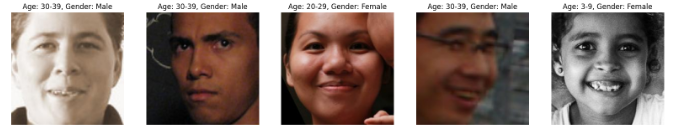
\includegraphics[width=\columnwidth]{graphics/randomtrain.png}
    \caption[5 willekeurige train voorbeelden]{5 willekeurige train voorbeelden met leeftijd en geslacht label}
        \label{fig:5randomtrain}}
\end{figure}

\section{Feature extractie} \label{sec:poc-featextractie}
De feature extractie is de eerste preprocessing stap in de machine learning pipeline. In deze Proof of Concept wordt het getrainde dlib model van \textcite{King2024} gebruikt. Dit model detecteert en voorspelt de 68 landmarks uit het gezicht. Het model is beschikbaar via GitHub en is beperkt in opslag. Doordat het model al voorgetraind is, hoeft dit dus niet opnieuw getraind te worden en versnelt het preprocessing proces. Door het detecteren van de landmarks kunnen we deze behouden en de afbeelding normaliseren, zoals in {~\ref{sub:normalisatie}}. \\
\\
\textcite{King2024} stelt ook een model ter beschikking waarop slechts 5 landmarks gedetecteerd worden. Dit zijn de 2 uiteinden van de ogen en het midden van de neus. Figuur ~\ref{fig:5landmarks} geeft een voorbeeld van een gezichtsafbeelding waarop deze 5 landmarks worden aangeduid. Voor deze use case zijn de 5 landmarks duidelijk te weinig om de volledige vorm van het gezicht weer te geven. Dit model met 5 landmarks is efficiënter bij een simpele gezichtsdetectie, om opslag te besparen en het model te versnellen.

\begin{figure}[H]
    \centering
    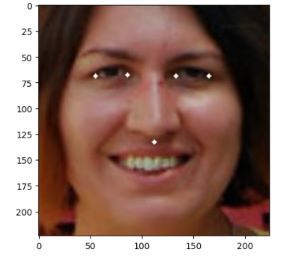
\includegraphics[width=\columnwidth]{graphics/5landmarks.PNG}
    \caption[5 landmarks op het gezicht]{5 landmarks op het gezicht}
    \label{fig:5landmarks}}
\end{figure}

\begin{enumerate}
    \item De eerste stap in dit proces omvat het detecteren van de 68 landmarks  \autocite{Serengil2020}. Deze omvatten de vorm van het gezicht, wenkbrauwen, ogen, neus en mond. Dit wordt uitgevoerd met het \textit{shape\_predictor\_68\_face\_landmarks} model van \textcite{King2024}. Vervolgens wordt de \textit{circle} functie van \textcite{OpenCV2024} gebruikt om de landmarks aan te duiden op de afbeelding. \\
    Figuur {~\ref{fig:68landmarks} geeft het resultaat van deze stap weer. \\
    \item Vervolgens wordt op basis van de gedetecteerde landmarks de vorm van het gezicht uit de afbeelding gehaald. De coördinaten van deze landmarks worden opgehaald en met \textit{line} van \textcite{OpenCV2024} omcirkeld. Er wordt een lijn getrokken van het eerste punt naar het volgende in de lijst met coördinaten. Figuur {~\ref{fig:gezichtsvorm}} geeft het resultaat van deze stap. \\ 
    \item Ten slotte maken we een mask voor de overgebleven afbeelding. Alles rond de vorm van het gezicht wordt met \textit{fillConvexPoly} van \textcite{OpenCV2024} zwart ingekleurd. Hierdoor wordt de onbelangrijke achtergrond van de afbeelding verwijdert en wordt enkel het gezicht overgehouden. Deze stap voert de normalisatie net zoals \textcite{Chen2011} uit, gebruikmakend van de HOG features in het detecteren van de landmarks, omschreven in  ~\ref{sub:hog}. Figuur {~\ref{fig:normalisatie}} geeft het resultaat van deze stap weer. Dit is een genormaliseerde afbeelding die gebruikt zal worden voor de feature dimensionaliteitsreductie.
\end{enumerate}\\

Het normaliseren van de afbeeldingen kan in een functie worden gestoken. Hierdoor kan aan de volledige dataset een mask toegevoegd worden, in plaats van slechts 1 afbeelding voordien. Het toevoegen van een mask aan een afbeelding duurt minder dan een seconde. Dit maakt deze methode geschikt voor de grote dataset.  Het toevoegen van de mask wordt in batches gedaan, om het proces te versnellen. Er wordt hierdoor steeds aan een aantal afbeeldingen tegelijk een mask toegevoegd, in plaats van 1 afbeelding per keer. Er wordt gekozen voor een batch size van 128, omdat deze voldoende groot is voor de beschikbare rekenkracht op een standaard laptop. Het volledige proces nam 84 minuten in beslag voor 86.744 afbeeldingen. \\
\\
Daarnaast kan deze functie ook valideren dat er geen duidelijke gezichten aanwezig zijn op de afbeeldingen, doordat de 68 landmarks niet gedetecteerd kunnen worden. Deze afbeeldingen zijn onbruikbaar en worden zo ook uit de dataset gehaald. Figuur {~\ref{fig:noface}} geeft een afbeelding weer waarop de landmarks niet gedetecteerd kunnen worden. Dit komt doordat de foto geen vooraanzicht is en op deze figuur zijn beide ogen niet duidelijk weergegeven.  Codevoorbeeld {~\ref{sc:mask} geeft deze functie weer \autocite{Serengil2020}. In de genormaliseerde trainingsdataset blijven nog 63.938 afbeeldingen over, in de genormaliseerde testset blijven nog 8.028 over. Beide datasets verliezen na normalisatie zo ongeveer 27\% van de gezichtsafbeeldingen, maar zijn nog voldoende groot om mee verder te werken.

\begin{figure}[H]
    \centering
    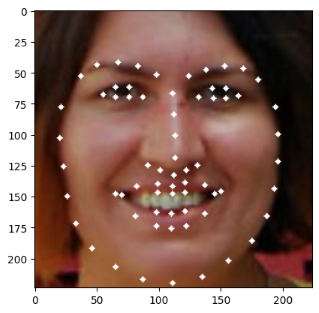
\includegraphics{graphics/68landmarks.png}
    \caption[68 landmarks op gezicht]{68 landmarks op het gezicht}
    \label{fig:68landmarks}}
\end{figure}

\begin{figure}[H]
    \centering
    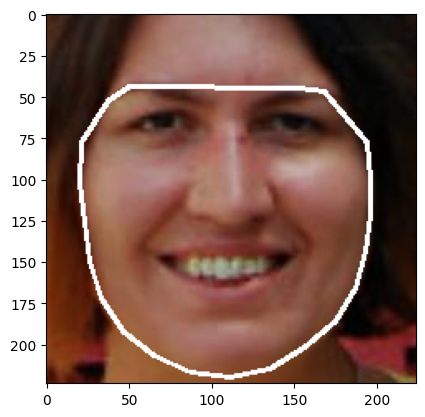
\includegraphics{graphics/gezichtsvorm.png}
    \caption[Gezichtsvorm uit afbeelding halen]{Gezichtsvorm uit afbeelding halen op basis van landmarks}
    \label{fig:gezichtsvorm}}
\end{figure}

\begin{figure}[H]
    \centering
    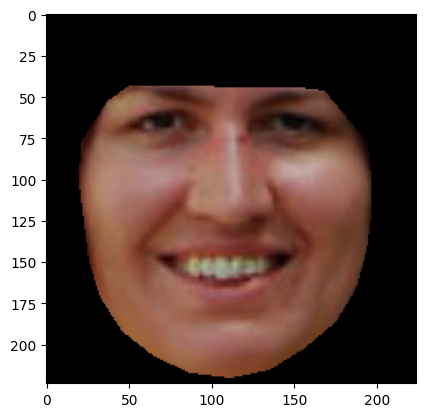
\includegraphics{graphics/normalisatie.png}
    \caption[Normalisatie van gezichtsafbeelding]{Normalisatie van gezichtsafbeelding}
    \label{fig:normalisatie}}
\end{figure}

\begin{lstlisting}[style=mystyle, caption={Functie om mask toe te voegen aan de volledige dataset \autocite{Serengil2020}}, label={sc:mask}]
import os
import cv2
import dlib
import numpy as np

def get_mask(image_paths, predictor_path, output_folder):
# Initialize face detector and landmark detector
face_detector = dlib.get_frontal_face_detector()
landmark_detector = dlib.shape_predictor(predictor_path)

for image_path in image_paths:
image = dlib.load_rgb_image(image_path)

# Detect faces in the image -> do not mask images where no face is found
faces = face_detector(image, 1)
no_faces = []
if len(faces) == 0:
print("No faces found in the image:", image_path)
no_faces.append(image_path)
continue

# Predict facial landmarks
face = faces[0] # only one face
landmarks = landmark_detector(image, face)
landmarks_tuple = [(landmarks.part(i).x, landmarks.part(i).y) for i in range(68)]

# Define the route for the mask
routes = [i for i in range(16,-1,-1)] + [i for i in range(17,19)] + [i for i in range(24,26)] + [16]
routes_coordinates = [landmarks_tuple[i] for i in routes]

# Create a mask
mask = np.zeros((image.shape[0], image.shape[1]), dtype=np.uint8)
mask = cv2.fillConvexPoly(mask, np.array(routes_coordinates), 255)
masked_image = cv2.bitwise_and(image, image, mask=mask)

# Save the masked image to the output folder with the same filename
filename = os.path.splitext(os.path.basename(image_path))[0]
output_filename = filename + "_masked.jpg"
output_path = os.path.join(output_folder, output_filename)
cv2.imwrite(output_path, masked_image)

print("Masked image saved:", output_path)

# Configuration
predictor_path = "./shape_predictor_68_face_landmarks.dat"
input_folder = 'data/train'
output_folder = './data/masked_train'
batch_size = 128

# Create the output folder if it doesn't exist
if not os.path.exists(output_folder):
os.makedirs(output_folder)

# List all image files in the input folder
image_files = sorted([f for f in os.listdir(input_folder) if f.endswith(('.jpg', '.jpeg', '.png'))], key=lambda x: int(os.path.splitext(x)[0]))

# Process images in batches
for i in range(0, len(image_files), batch_size):
batch_images = image_files[i:i+batch_size]
batch_paths = [os.path.join(input_folder, image) for image in batch_images]
get_mask(batch_paths, predictor_path, output_folder) 
\end{lstlisting} 
\begin{figure}
    \centering
    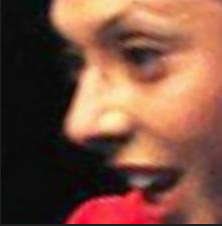
\includegraphics{graphics/no_face_detected.png}
    \caption[Geen gezicht gedecteerd op afbeelding]{De 68 landmarks werden niet teruggevonden op de gezichtsafbeelding, deze wordt verwijderd uit de dataset.}
    \label{fig:noface}}
\end{figure}

% ---- Feature dim
\section{Feature dimensionaliteitsreductie}\label{sec:poc-featuredim}
Op de genormaliseerde afbeeldingen wordt Truncated SVD toegepast als dimensionaliteitsreductie van de features. Doordat de dataset zeer veel afbeeldingen bevat, wordt geopteerd voor Truncated SVD in plaats van het gekende PCA. PCA vereist een enorme rekenkracht op een grote dataset, omdat deze de covariantie van de matrix van de originele dataset berekent. Truncated SVD berekent de singular value decomposition van de datamatrix, wat veel efficiënter is voor grote en sparse datasets \autocite{Baruah2023}. De benodigde opslag zal verminderen en de impact van noise op de dataset daalt. Het uitvoeren van PCA op de dataset, of zelfs een subset daarvan, genereert meteen een foutmelding over de benodigde opslag. Een standaard laptop kan deze berekening niet aan.\\
\\
De Truncated SVD functie wordt beschikbaar gesteld via \textit{sklearn.decomposition}. Aan Truncated SVD wordt het aantal componenten, dat behouden moet worden, als paramater meegegeven. Dit is de gewenste dimensionaliteit van de output data. De dimensionaliteit moet steeds minder zijn dan het aantal features in de data \autocite{ScikitLearn2024}. Het ideale aantal componenten kan berekend worden aan de hand van de verklaarde variantie. Er wordt een lus gemaakt door de Truncated SVD met een range die gaat tot de shape van de trainingsdata. Voor elk aantal componenten wordt de verklaarde variantie berekend. De grafiek met de verklaarde variantie per aantal componenten kan teruggevonden worden op figuur {~\ref{fig:explainedvar}}. \\
\\ 
Er wordt verder gewerkt met 400 componenten, omdat deze een verklaarde variantie van circa 0.99 heeft. Hierdoor daalt het aantal componenten van de data van 1000 naar 400. De features van data worden zo gereduceerd om makkelijker mee verder te werken bij het trainen van de machine learning modellen. Codevoorbeeld {~\ref{sc:truncatedsvd} geeft weer hoe de Truncated SVD wordt toegepast op de volledige trainingsdataset. Het resultaat van de dimensionaliteitsreductie op een gezichtsafbeelding is te vinden op figuur {~\ref{fig:truncated}}.
\begin{figure}[H]
    \centering
    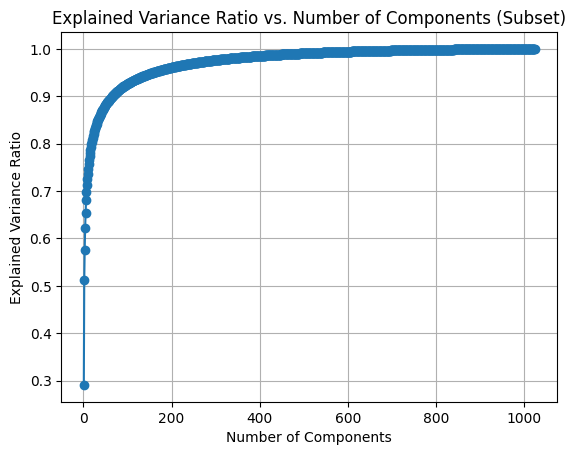
\includegraphics{graphics/explained_variance.png}
    \caption[Verklaarde variantie voor de Truncated SVD]{Verklaarde variantie voor de Truncated SVD}
    \label{fig:explainedvar}}
\end{figure}
\begin{lstlisting}[style=mystyle, caption={Functie om Truncated SVD toe te passen op de volledige dataset \autocite{ScikitLearn2024}}, label={sc:truncatedsvd}]
% Apply TruncatedSVD for dimensionality reduction
svd = TruncatedSVD(n_components=400)
X_train_svd = svd.fit_transform(X_train)  
\end{lstlisting}
\begin{figure}[H]
    \centering
    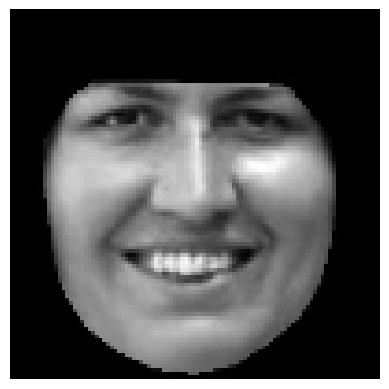
\includegraphics{graphics/truncatedsvd.png}
    \caption[Truncated SVD toegepast op genormaliseerde gezichtsafbeelding]{Truncated SVD toegepast op genormaliseerde gezichtsafbeelding}
    \label{fig:truncated}}
\end{figure}

\section{Machine learning modellen}\label{sec:poc-mlmodellen}
Om het meest geschikte machine learning model te vinden voor de voorspelling van leeftijd en geslacht op basis van gezichtsafbeeldingen, worden verschillende modellen uit de literatuurstudie in hoofdstuk ~\ref{sec:bestaandeml} getest. De performantie van 2 aparte modellen die leeftijd en geslacht voorspellen, alsook 1 model die beide voorspelt worden geanalyseerd. \\
\\
Om optimaal te zoeken naar de beste parameters wordt gebruik gemaakt van GridSearch ~\ref{sub:gridsearch}. Hieraan worden meerdere parameters meegegeven, zoals aantal estimators of kernel, waarvoor GridSearch de parameter met de beste score na training weergeeft. Aan de parameters van Grid Search wordt 5 als standaardwaarde van de cross validatie meegegeven. Zoals in ~\ref{sub:gridsearch} aangehaald, worden er 5 herhalingen uitgevoerd op de dataset om het model te optimaliseren. De modellen met hun parameters worden geëvalueerd op basis van de balanced accuracy. Deze score gaat het aantal correct voorspelde instanties na, in een dataset die mogelijks ongelijk verdeeld is \autocite{Garcia2009}. Tabel ~\ref{tab:leeftijdcat} geeft weer hoe de leeftijdscategorieën verdeeld zijn en tabel ~\ref{tab:geslacht} hoe geslacht verdeeld is in de trainingsdata. Hieruit kan afgeleid worden dat de leeftijdscategorieën niet even verdeeld zijn en dat balanced accuracy hier wel degelijk de betere optie is. \\
\\
De testfase van de GridSearch wordt uitgevoerd op een subset van 1000 willekeurige afbeeldingen uit de dataset om de tijd die nodig is om te trainen te verminderen. Het model met de parameters die de beste score leveren, wordt dan uiteindelijk getraind op de volledige trainingsdataset. \\
\begin{center}
    \caption{Verdeling van leeftijdscategorieën}
    \label{tab:leeftijdcat}
    \begin{tabular}{||c | c | c||} 
        \hline
        Leeftijdscategorie & Aantal & Percentage van volledige dataset  \\ 
        \hline
        0-2 & 1399 & 2,19\% \\
        \hline
        3-9 & 8003 & 12,52\% \\
        \hline
        10-19 & 6880 & 10,76\% \\
        \hline
        20-29 & 18924 & 29,60\% \\
        \hline 
        30 -39 & 13874 & 21,70\% \\
        \hline
        40-49 & 7726 & 12,08\% \\
        \hline 
        50-59 & 4528 & 7,08\% \\
        \hline 
        60-69 & 1980 & 3,10\% \\
        \hline 
        more than 70 & 624 & 1\% \\
    \end{tabular}
\end{center}

\begin{center}
     \caption{Verdeling van geslacht}
       \label{tab:geslacht}
    \begin{tabular}{||c | c | c||} 
        \hline
        Geslacht & Aantal & Percentage van volledige dataset  \\ 
        \hline
        Male & 32435 & 50,73\% \\
        \hline
        Female & 31503 & 49,27\% \\
        
    \end{tabular}
\end{center}

\\
Om een model te trainen die beide (leeftijd en geslacht) gelijktijdig kan voorspellen, wordt gebruik gemaakt van de MultiOutputClassifier van \textit{sklearn.multioutput}. Deze strategie bestaat uit het aanpassen van een classifier per target. Hiermee kunnen classifiers uitgebreid worden die van nature geen multi-target classificatie ondersteunen, zoals Random Forest Classifier \autocite{ScikitLearn2024}. Het model geeft als output 2 labels, één voor geslacht en één voor de leeftijdscategorie. \\
\\ 
Het getrainde model wordt getest op de validatie dataset. Dit gebeurt met de \textit{predict} functie van Scikit-learn. Op basis hiervan wordt de confusion matrix opgesteld en de performantiescores, aangehaald in de literatuurstudie ~\ref{ch:standvanzaken}, berekent. \textcite{ScikitLearn2024} heeft al enkele ingebouwde functies om de performantiescores, zoals $accuracy\_score$ en $precison\_score$, te berekenen. Deze kunnen uitgevoerd worden op de confusion matrix van het geslacht. Voor de modellen die leeftijd en beide voorspellen dienen de scores handmatig berekend te worden, omdat dit geen 2x2 matrices zijn. 

\subsection{Random Forest Classifier} \label{sub:poc-rfc}
Het Random Forest Classifier model wordt beschikbaar gesteld via \textit{sklearn.ensemble}.
Omdat het model geen tekstuele data kan categoriseren, dienen de labels omgezet te worden naar numerische waarden. Voor het geslacht (Female of Male) wordt dit 0 of 1. Voor de leeftijdscategorieën wordt OrdinalEncoder gebruikt om deze te mappen naar een getal tussen 0 en 8, waarbij '0-2' categorie 0 wordt en 'more than 70' categorie 8 wordt. Aan deze Ordinal Encoder geven we een mapping mee van de labels. De encoder gaat deze dan fitten op de gegeven labels van de dataset volgens de meegegeven mapping \autocite{ScikitLearn2024}.  \\
\\
Aan de Grid Search voor de Random Forest Classifier worden volgende parameters meegegeven:
\begin{itemize}
    \item $n\_estimators$: het aantal bomen dat gebruikt wordt (default = 100). 
    \item $max\_features$: het aantal features die gebruikt worden om de beste scheiding in de bomen te vinden (default = 'sqrt')
    \item $min\_samples\_split$: het minimum aantal instanties die nodig zijn om node te mogen splitsen (default = 2).
    \item $min\_samples\_leaf$: minimum aantal instanties die in een blad moeten zitten (default = 1). Een blad is het uiteinde van een boom, die de voorspelde klasse weergeeft \textcite{Garg2020}. 
    \item $max\_depth$: de maximale diepte van een boom (default = None). 
    \item bootstrap: het gebruik van steekproeven bij het bouwen van de bomen (default = True)
\end{itemize}
\\
\begin{center}
    \begin{tabular}{||c | c  | c | c||} 
        \hline
          & Geslacht & Leeftijd & Beide  \\ 
        \hline
        Parameters & $n\_estimators=230$ & $max\_depth$=5, $n\_estimators$=200 & $n\_estimators$=100  \\ 
        \hline
        Accuracy & 99,99\% & 29,71\% & 99,95\%  \\
        \hline
        Precision & 99,99\% & 0,00\% & 99,93\%  \\
        \hline
        Recall & 100\% & 11,21\% & 99,92\%  \\
        \hline
        Specificity & 99,99\% & 0,00\% & 99,99\% \\
        \hline
        F1 & 99,99\% & 0.00\% & 99,93\%  \\
    \end{tabular}
\end{center}
\\
\\
Figuur ~\ref{fig:cmrfc} geeft de confusion matrices voor de 3 modellen weer. Uit de confusion matrices en de scores kunnen we afleiden dat de Random Forest Classifier uitstekend presteert voor de voorspelling van geslacht en beide. Voor de voorspelling van de leeftijdscategorie behaalt dit model slechts een score van circa 30\%. Uit de confusion matrix van de leeftijdsvoorspellingen is ook af te leiden dat vrijwel enkel de leeftijdscategorie 20-29 wordt voorspelt. Dit kan te verklaren zijn door overfitting, omdat deze klasse het meest aanwezig is in de dataset is de kans het grootst dat de voorspelling juist is \autocite{Kreiger2020}. Het model presteert wel goed wanneer het geslacht ook wordt toegevoegd. Dit kan te verklaren zijn door de levensfactoren en opvoeding, aangehaald in ~\ref{sec:voorspellen}. Het model krijgt de context van het geslacht mee en kan hierdoor wel patronen herkennen. \\
\begin{figure}[H]
    \centering
    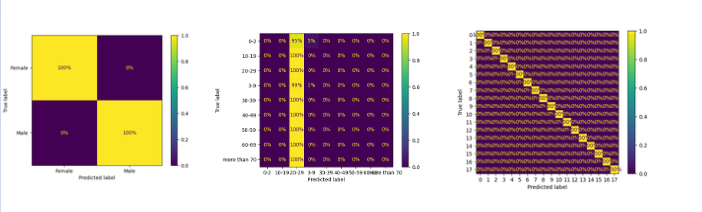
\includegraphics{graphics/cm_rfc.png}
    \caption[Confusion Matrix voor Random Forest Classifier]{Confusion Matrix voor Random Forest Classifier}
    \label{fig:cmrfc}}
\end{figure}

\subsection{XGBoost Classifier} \label{sub:poc-xgb}
Het XGBoost, Extreme Gradient Boosting, Classifier model wordt beschikbaar gesteld via \textit{xgboost}. Ook aan dit model kan geen tekstuele data worden meegeven en worden de labels omgezet in numerische waarden, zoals in ~\ref{sub:poc-rfc}. \\
\\
Voor de classificatie van beide labels met de MultiOutputClassifier vindt nog een preprocessing stap plaats. De tekstuele labels moeten omgezet worden naar numerische categorieën. Hiervoor wordt de LabelEncoder van \textit{sklearn.preprocessing} gebruikt. De labels worden dan samengevoegd met \textit{$np.column\_stack$}. Codevoorbeeld ~\ref{sc:prepmulti} geeft weer hoe de labels worden aangepast voor de MultiOuputClassifier. Het label voor een vrouwelijke 0-2 jarige wordt zo [0,1]. \\
\\
Aan de Grid Search voor de XGBoost Classifier worden volgende parameters meegegeven: 
\begin{itemsize}
    \item $n\_estimators$: het aantal bomen dat gebruikt wordt (default = 100). 
    \item $max\_depth$: de maximale diepte van een boom (default = 6). 
\end{itemsize}

\begin{lstlisting}[style=mystyle, caption={Functie om labels aan te passen voor de MultiOutputClassifier \autocite{Roepke2024} en \autocite{Numpy2024}}, label={sc:prepmulti}]
        age_class_encoded = label_encoder.fit_transform(y_train_age)
        gender_encoded = label_encoder.fit_transform(y_train_gender)
        y_combined = np.column_stack((age_class_encoded, gender_encoded))
    \end{lstlisting}

\begin{center}
    \begin{tabular}{||c | c | c | c||} 
        \hline
        & Geslacht & Leeftijd & Beide  \\ 
        \hline
        Parameters & $n\_estimators=267$, $depth$=5 &  $n\_estimators$=300, $depth$=4 & $n\_estimators$=100 \\ 
        \hline
        Accuracy & 94.76\% & 81,82\% & 10,23\%  \\
        \hline
        Precision & 95.22\% & 90,98\% & 6,50\%  \\
        \hline
        Recall & 94.09\% & 84,16\% & 5,35\% \\
        \hline
        Specificity & 95.41\% & 97,30\% & 94,32\% \\
        \hline
        F1 & 94.65\% & 87,44\% & 5,87\%  \\
      
    \end{tabular}
\end{center}
\\
\\
Figuur ~\ref{fig:cmxgb} geeft de confusion matrices voor de XGBoost classifier modellen weer. Hieruit kunnen we afleiden dat de XGBoost Classifier zeer goed presteert voor de aparte voorspelling van leeftijd en geslacht. Wanneer beide labels gelijktijdig worden voorspeld, presteert het model zeer slecht. Ook dit kan te verklaren zijn door overfitting, de aard van de data of het model kan geen patronen vinden. 

\begin{figure}[H]
    \centering
    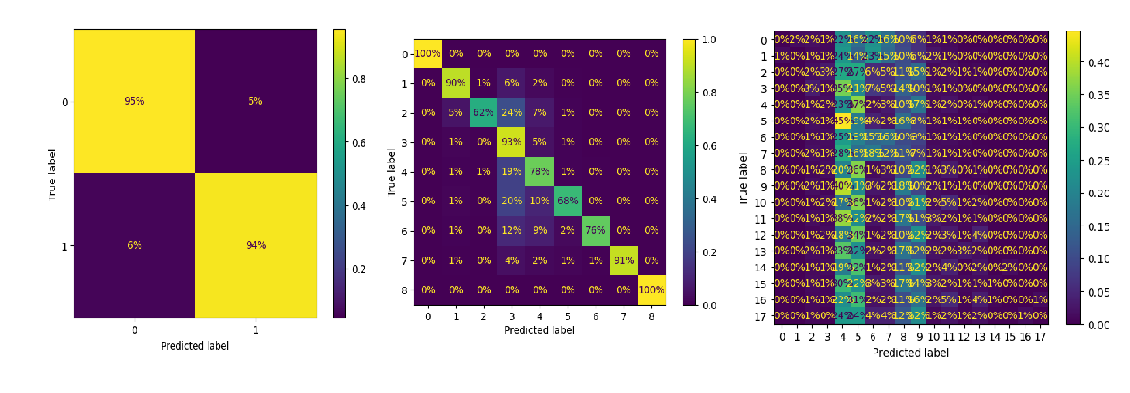
\includegraphics[width=\columnwidth]{graphics/cm_xgb.png}
    \caption[Confusion Matrix voor XGBoost Classifier]{Confusion Matrix voor XGBoost Classifier}
    \label{fig:cmxgb}}
\end{figure}
\subsection{Support Vector Machines} \label{sub:poc-svm}
Het Support Vector Classifier (SVC) model wordt beschikbaar gesteld via \textit{sklearn.svm}. Een SVM kan wel classificeren op basis van tekstuele data. Aan dit model wordt wel de originele dataset meegegeven en worden de labels niet gewijzigd. \\
\\
Aan de Grid Search voor het SVC model worden volgende parameters meegegeven:
\begin{itemize}
    \item C: regularisatie parameter, afhankelijk van de grootte van de dataset (default = 1.0).
    \item gamma: coëfficiënt van de kernel (default = 'scale')
    \item kernel: kernel type die gebruikt wordt in het algoritme (default = 'rbf').
    \item degree: graad van de kernel (default = 3).
\end{itemize}
\begin{center}
    \begin{tabular}{||c | c | c | c||} 
        \hline
        & Geslacht & Leeftijd & Beide  \\ 
        \hline
        Parameters & C=125 &  C=125, kernel='linear', degree=1 & C=25  \\ 
        \hline
        Score model (train) & 68.41\% & 21.52\% & 20.50\%  \\
        \hline
        Accuracy & 66.79\% & 28.23\% & 21.55\%  \\
        \hline
        Precision & 67.57\% & 22.12\% & 19.44\%  \\
        \hline
        Recall & 66.40\% & 21.70\% & 13.87\%  \\
        \hline
        Specificity & 67.19\% & 90.17\% & 95.15\% \\
        \hline
        F1 & 66.98\% & 21.91\% & 16.18\%  \\
       
    \end{tabular}
\end{center}
\\
\\
Figuur ~\ref{fig:svc} geeft de confusion matrices voor de SVC modellen weer. Uit de scores kan afgeleid worden dat het SVC model slechter presteert dan voorgaande modellen. Voor de voorspelling van geslacht wordt hier slechts een score van circa 70\% behaald. Ook de modellen voor de voorspelling van leeftijd en beide presteren slecht, met een score van slechts 20\%. Ook uit de confusion matrices is af te leiden dat er veel foute voorspellingen zijn. Hieruit kan geconcludeerd worden dat een SVC niet het geschikte model is voor de classificatie van gezichtsafbeeldingen. 
\\
\begin{figure}[H]
    \centering
    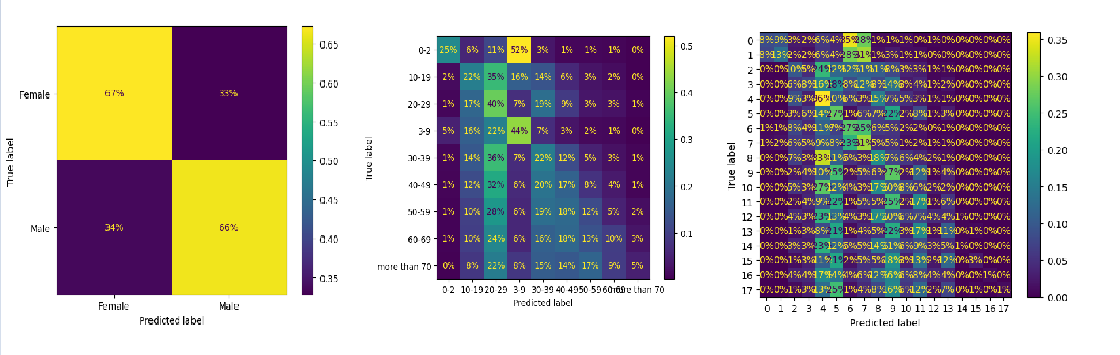
\includegraphics[width=\columnwidth]{graphics/cm_svc.png}
    \caption[Confusion Matrix voor Support Vector Classifier]{Confusion Matrix voor Support Vector Classifier}
    \label{fig:svc}}
\end{figure}
\subsection{Voting Classifier} \label{sub:poc-votingclass}
De Voting Classifier is een ensemble techniek die meerdere modellen combineert. De SVC, random forest en XGBoost Classifier worden tegelijk aangesproken om de accuracy van het model te verhogen. De parameters die het beste scoorden voor de afzonderlijke modellen worden hier hergebruikt. Codevoorbeeld ~\ref{?} geeft weer hoe de Voting Classifier de verschillende modellen combineert. 

\begin{center}
    \begin{tabular}{||c c c c||} 
        \hline
        & Geslacht & Leeftijd & Beide  \\ 
        \hline
        Parameters & ? &  ? & ?  \\
        \hline
        Accuracy & ?\% & ?\% & ?\%  \\
        \hline
        Precision & ?\% & ?\% & ?\%  \\
        \hline
        Recall & ?\% & ?\% & ?\%  \\
        \hline
        Specificity & ?\% & ?\% & ?\% \\
        \hline
        F1 & ?\% & ?\% & ?\%  \\
        
    \end{tabular}
\end{center}
    %...
    
    %%=============================================================================
%% Conclusie
%%=============================================================================

\chapter{Conclusie}%
\label{ch:conclusie}

% TODO: Trek een duidelijke conclusie, in de vorm van een antwoord op de
% onderzoeksvra(a)g(en). Wat was jouw bijdrage aan het onderzoeksdomein en
% hoe biedt dit meerwaarde aan het vakgebied/doelgroep? 
% Reflecteer kritisch over het resultaat. In Engelse teksten wordt deze sectie
% ``Discussion'' genoemd. Had je deze uitkomst verwacht? Zijn er zaken die nog
% niet duidelijk zijn?
% Heeft het onderzoek geleid tot nieuwe vragen die uitnodigen tot verder 
%onderzoek?

\lipsum[76-80]


    
    %---------- Bijlagen -----------------------------------------------------------
    
    \appendix
    
    \chapter{Onderzoeksvoorstel}
    
    Het onderwerp van deze bachelorproef is gebaseerd op een onderzoeksvoorstel dat vooraf werd beoordeeld door de promotor. Dat voorstel is opgenomen in deze bijlage.
    
    %% TODO: 
    \section*{Samenvatting}
    
    % Kopieer en plak hier de samenvatting (abstract) van je onderzoeksvoorstel.
    Gezichtsanalyse heeft de laatste jaren veel aandacht gekregen vanwege de brede toepassingen op verschillende gebieden, zoals gezondheidszorg, beveiliging en marketing.  
    De focus van de bachelorproef ligt op het ontwikkelen en implementeren van een robuust systeem voor het schatten van leeftijd en geslacht op basis van gezichtsfoto’s, met behulp van machine learning technieken. Dit onderzoek is van bijzonder belang voor het verbeteren van de beoordeling van geestelijke gezondheidszorg door camera-gebaseerde gezondheidsmetingen. Deze inspanningen dragen bij aan de doelstellingen van IntelliProve, een platform dat online gezondheidsoplossingen biedt. Er wordt onderzocht welke machine learning technieken de beste resultaten tonen en uit welke elementen de volledige pipeline zal bestaan.   
    In de eerste fase van het onderzoek wordt een literatuurstudie uitgevoerd om uit bestaand onderzoek de gebruikte modellen te verkennen en hun sterktes, limitaties en performantie te achterhalen. In de proof-of-concept gebeurt eerst de preprocessing, feature extractie en gezichtsdetectie. Daarna worden de modellen uit de literatuurstudie getest op bestaande datasets en wordt een prestatie-evaluatie opgesteld op basis van metrieken zoals accuracy, precision, recall, F1-score en ROC curve. Het verwachte resultaat is een robuuste machine learning pipeline waarmee IntelliProve de leeftijd en het geslacht kan voorspellen op basis van een gezichtsafbeelding. 
    
    % Verwijzing naar het bestand met de inhoud van het onderzoeksvoorstel
    %---------- Inleiding ---------------------------------------------------------

\section{Introductie}%
\label{sec:introductie}

De onderzoeksvraag werd aangeboden door het bedrijf IntelliProve. IntelliProve biedt online gezondheidsoplossingen, een software die in staat is om binnen enkele seconden nauwkeurig gezondheidsparameters te bepalen, gebaseerd op een optische meting van het gezicht.  
Het doel van de bachelorproef is het ontwikkelen en implementeren van een robuust systeem voor het schatten van de leeftijd en het geslacht van personen op basis van gezichtsfoto's, met behulp van machine learning-technieken. 
Dit project is van bijzonder belang voor het verbeteren van de beoordeling van de geestelijke gezondheidszorg door middel van camera-gebaseerde gezondheidsmetingen. Het onderzoek beoogt bij te dragen aan de vooruitgang op dit gebied door gebruik te maken van geavanceerde algoritmen om leeftijd en geslacht nauwkeurig te voorspellen aan de hand van gezichtsbeelden.  
De literatuurstudie biedt een inzicht in facial analysis, de bestaande machine learning modellen en hun functionaliteiten. De proof-of-concept zal bestaan uit het ontwikkelen van een machine learning pipeline dat in staat is om leeftijd en geslacht te voorspellen op basis van bestaande datasets. De pipeline omvat verschillende image preprocessing technieken om de dataset voor te bereiden op de modeltraining. Om betrouwbaarheid en accuracy te garanderen, worden de modellen verfijnd en geoptimaliseerd om de hoogst mogelijke nauwkeurigheid te bereiken bij het schatten van leeftijd en geslacht.

\section{State-of-the-art}%
\label{sec:state-of-the-art}

Hier beschrijf je de \emph{state-of-the-art} rondom je gekozen onderzoeksdomein, d.w.z.\ een inleidende, doorlopende tekst over het onderzoeksdomein van je bachelorproef. Je steunt daarbij heel sterk op de professionele \emph{vakliteratuur}, en niet zozeer op populariserende teksten voor een breed publiek. Wat is de huidige stand van zaken in dit domein, en wat zijn nog eventuele open vragen (die misschien de aanleiding waren tot je onderzoeksvraag!)?

Je mag de titel van deze sectie ook aanpassen (literatuurstudie, stand van zaken, enz.). Zijn er al gelijkaardige onderzoeken gevoerd? Wat concluderen ze? Wat is het verschil met jouw onderzoek?

Verwijs bij elke introductie van een term of bewering over het domein naar de vakliteratuur, bijvoorbeeld~\autocite{Hykes2013}! Denk zeker goed na welke werken je refereert en waarom.

Draag zorg voor correcte literatuurverwijzingen! Een bronvermelding hoort thuis \emph{binnen} de zin waar je je op die bron baseert, dus niet er buiten! Maak meteen een verwijzing als je gebruik maakt van een bron. Doe dit dus \emph{niet} aan het einde van een lange paragraaf. Baseer nooit teveel aansluitende tekst op eenzelfde bron.

Als je informatie over bronnen verzamelt in JabRef, zorg er dan voor dat alle nodige info aanwezig is om de bron terug te vinden (zoals uitvoerig besproken in de lessen Research Methods).

% Voor literatuurverwijzingen zijn er twee belangrijke commando's:
% \autocite{KEY} => (Auteur, jaartal) Gebruik dit als de naam van de auteur
%   geen onderdeel is van de zin.
% \textcite{KEY} => Auteur (jaartal)  Gebruik dit als de auteursnaam wel een
%   functie heeft in de zin (bv. ``Uit onderzoek door Doll & Hill (1954) bleek
%   ...'')

Je mag deze sectie nog verder onderverdelen in subsecties als dit de structuur van de tekst kan verduidelijken.

%---------- Methodologie ------------------------------------------------------
\section{Methodologie}%
\label{sec:methodologie}

\subsection{Requirements}
\label{sub:requirements}
In de eerste week wordt nagevraagd aan belanghebbenden van IntelliProve aan welke criteria de modellen moeten voldoen. Alle data (gezichtsfoto's) worden verzameld. Er wordt onder andere nagegaan over welke functionaliteiten de modellen moeten beschikken en wat de verwachte prestatievereisten zijn. 
Als resultaat verwerven we een lijst van alle functionele en niet-functionele requirements, geordend volgens belang. 

\subsection{Literatuurstudie}
\label{sub:literatuurstudie}
De literatuurstudie omvat een diepgaande verkenning van facial analysis technieken en machine learning modellen. 
Deze fase biedt inzicht in de verschillende methoden voor het extraheren van gezichtskenmerken en image preprocessing technieken, specifiek met betrekking tot het schatten van leeftijd en geslacht.
Het doel is om kennis uit bestaand onderzoek te vergaren om effectieve methodologieën te identificeren in de huidige benaderingen van facial analysis. 
Het eindresultaat van deze fase, die 3 weken duurt, is een samenvatting van de belangrijkste bevindingen uit de literatuurstudie, die als basis zal dienen voor de proof-of-concept.
\subsection{Proof-of-concept}
\label{sub:proof-of-concept}
Deze fase start met het verzamelen en analyseren van de datasets. Technieken zoals normalisatie, scaling, feature-extractie en data augmentation worden gebruikt om de dataset voor te bereiden op modeltraining.
Vervolgens worden verschillende machine learning algoritmen geselecteerd op basis van de bevindingen uit de literatuurstudie. De modellen worden getraind en geëvalueerd op basis van de vooropgestelde requirements. 
De pipeline wordt beoordeeld op betrouwbaarheid en precisie op basis van de opgestelde requirements. Metrieken zoals accuracy, precision, recall, F1-score en ROC-curves worden gebruikt om de modellen te evalueren.
Er worden cross-validatie technieken gebruikt om de robuustheid van de modellen en de generalisatie van nieuwe data te testen. 
Deze fase vereist dan ook veel tijd en zal 6 weken duren. Het resultaat van deze fase is een proof-of-concept die bestaat uit een machine learning pipeline, die stappen voor het preprocessen van gegevens en getrainde modellen integreert voor het schatten van leeftijd en geslacht op basis van gezichtsfoto's.

\subsection{conclusie}
\label{sub:conclusie}
In de conclusiefase worden de resultaten van de evaluatie grondig geanalyseerd. De prestaties van de ontwikkelde modellen worden beoordeeld, waarbij hun sterke punten en beperkingen worden benadrukt. Het belang van een nauwkeurige schatting van leeftijd en geslacht bij de beoordeling van de geestelijke gezondheid en de implicaties voor de gezondheidszorg worden besproken. Er worden aanbevelingen gedaan voor mogelijke verbeteringen of toekomstige onderzoeksrichtingen op basis van de bevindingen en beperkingen van het project.
\subsection{Afwerken scriptie}
\label{sub:afwerken_scriptie}
De laatste fase, die 2 weken duurt, omvat het afwerken van de bachelorproef. Dit is het eindresultaat van het geleverde onderzoek met een proof-of-concept die zal worden ingediend. 


%---------- Verwachte resultaten ----------------------------------------------
\section{Verwacht resultaat, conclusie}%
\label{sec:verwachte_resultaten}

Hier beschrijf je welke resultaten je verwacht. Als je metingen en simulaties uitvoert, kan je hier al mock-ups maken van de grafieken samen met de verwachte conclusies. Benoem zeker al je assen en de onderdelen van de grafiek die je gaat gebruiken. Dit zorgt ervoor dat je concreet weet welk soort data je moet verzamelen en hoe je die moet meten.

Wat heeft de doelgroep van je onderzoek aan het resultaat? Op welke manier zorgt jouw bachelorproef voor een meerwaarde?

Hier beschrijf je wat je verwacht uit je onderzoek, met de motivatie waarom. Het is \textbf{niet} erg indien uit je onderzoek andere resultaten en conclusies vloeien dan dat je hier beschrijft: het is dan juist interessant om te onderzoeken waarom jouw hypothesen niet overeenkomen met de resultaten.


    
    %%---------- Andere bijlagen --------------------------------------------------
    % TODO: Voeg hier eventuele andere bijlagen toe. Bv. als je deze BP voor de
    % tweede keer indient, een overzicht van de verbeteringen t.o.v. het origineel.
    %\input{...}
    
    %%---------- Backmatter, referentielijst ---------------------------------------
    
    
    \backmatter{}
    
    \setlength\bibitemsep{2pt} %% Add Some space between the bibliograpy entries
    \printbibliography[heading=bibintoc]
    
\end{document}
